% Section content template for individual Educative lessons
% This file contains the actual content for a specific section
% Generated from Educative API section content

% Section: Sequence Diagram for the Airline Management System
% Section ID: 5450949964595200
% Section Slug: sequence-diagram-for-the-airline-management-system
% Generated: 2025-12-14T13:17:54.199613

Sequence diagrams are an effective way to visualize the interactions between different entities and objects within a system. We can create different sequence diagrams for our airline management system. In this lesson, we will create sequence diagrams for the following two interactions:

\begin{itemize}
\item
\protect\phantomsection\label{FUA-FPxZZMi_9rmpw6hvX}
\textbf{Reserve a flight:}~The customer reserves a flight online.
\item
\protect\phantomsection\label{pZhxItrr5lJhaJfKGVrnX}
\textbf{Sequence challenge:}~Assign a seat via \texttt{FrontDeskOfficer}.
\end{itemize}

\subsection{Reserve a flight}\label{RK5dqDlX75q-YAh-2yDoy}
\\
The sequence diagram for reserving a flight should have the following actors and objects that will interact with each other:

\begin{itemize}
\item
\protect\phantomsection\label{PvHaeAAsKo-rNbwYAP6Ds}
\textbf{Actor:}~\texttt{Customer}
\item
\protect\phantomsection\label{8v3mrbBn42GPFxaxLjNrn}
\textbf{Objects:}~\texttt{SearchCatalog},~\texttt{FlightInstance},~\texttt{FlightSeat}, \texttt{FlightReservation}, \texttt{Itinerary}, \texttt{Payment}, \texttt{SmsNotification}, and \texttt{EmailNotification}.
\end{itemize}
\\
Here are the steps in the reserve flight interaction:

\begin{enumerate}
\item
\protect\phantomsection\label{_6U_ei_c71qnd1fBODkqS}
The customer searches for flights flying from an airport on a particular date.
\item
\protect\phantomsection\label{3QjE2kASZiUMWuWxpk9GE}
The catalog returns a list of flights that satisfy the search query.
\item
\protect\phantomsection\label{wpg45-n9THKNOp0JpCrvu}
The customer selects a flight.
\item
\protect\phantomsection\label{v2L8JaQrajQ_y18TOBDRq}
Customer creates a reservation.
\item
\protect\phantomsection\label{GJWADVwzxBcUMg9oBsvla}
Customer creates an itinerary.
\item
\protect\phantomsection\label{SrVLsD772hPtu4yfwO0n3}
System requests payment.
\item
\protect\phantomsection\label{8KjmzBO-zqADGbmRYikPM}
Customer makes payment.
\item
\protect\phantomsection\label{IrAsEG7Tm7nleD2wom4Su}
Customer notified.
\end{enumerate}
\begin{quote}
\textbf{Note:} We assume that the customer performs a valid operation and successfully reserves the seat.
\end{quote}
\\
Based on the order above, the sequence diagram for reserving a flight in the airline management system is given below.

\begin{figure}[htbp]
 \centering
 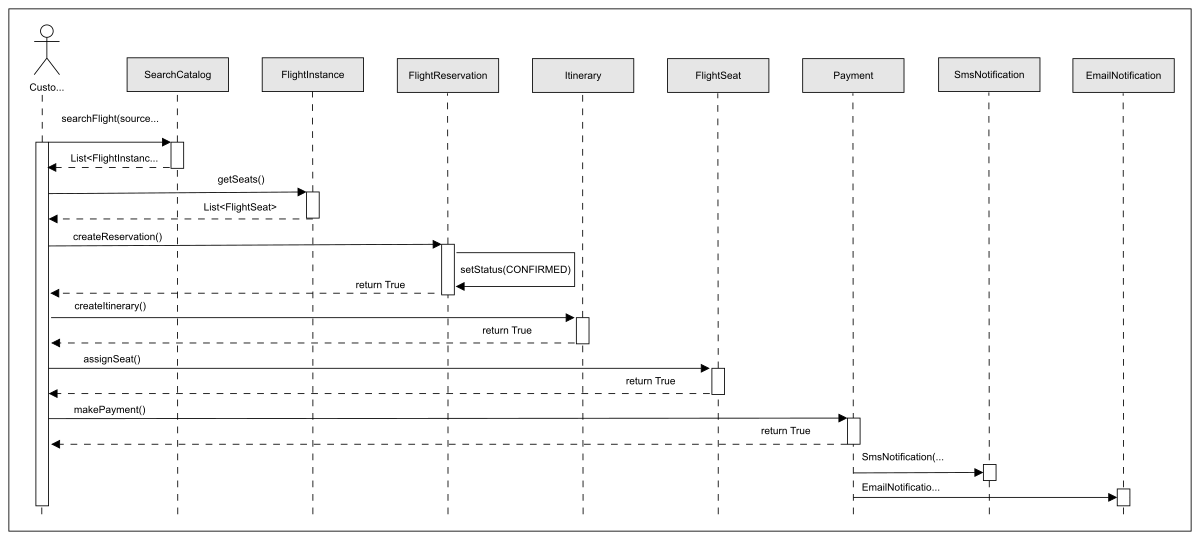
\includegraphics[width=0.5\textwidth]{Images/chapter_25/section_5450949964595200/5255035200864256.png}
 \caption{The sequence diagram for the “Reserve a flight” interaction}
\end{figure}

\subsection{Sequence challenge: Assign seat via FrontDeskOfficer}\label{EmiyaoQIJI8d-iTODhUJ3}
\\
Let's complete a sequence diagram for assigning a seat via \texttt{FrontDeskOfficer}. A skeleton of the sequence diagram is given below:

\begin{figure}[htbp]
 \centering
 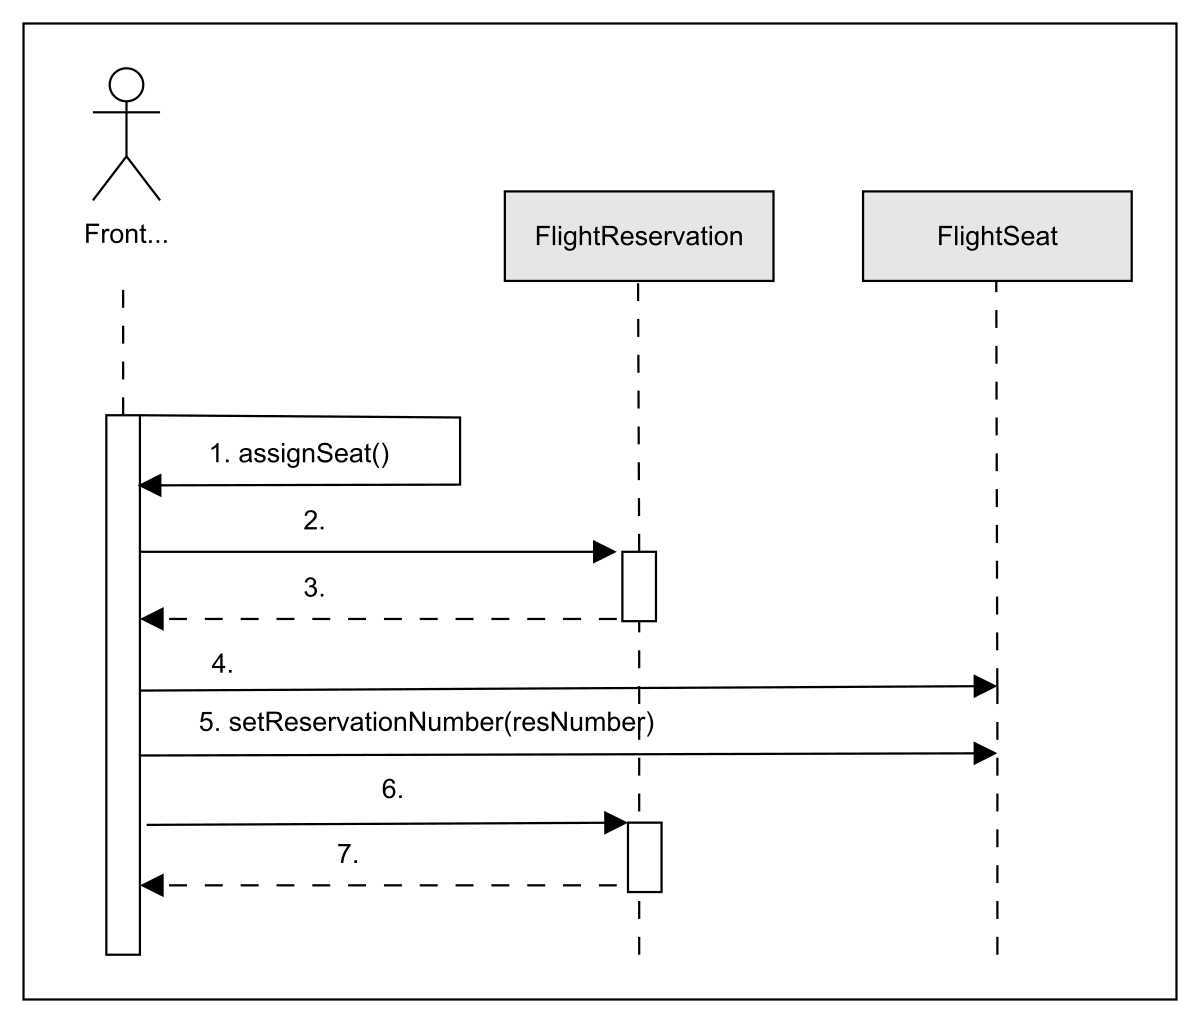
\includegraphics[width=0.5\textwidth]{Images/chapter_25/section_5450949964595200/4858354760286208.png}
 \caption{The sequence diagram for assigning a seat via FrontDeskOfficer}
\end{figure}

Notice that the arrows in the diagram above are numbered from 1 to 7. The message boxes shown below are the messages to be exchanged between the actor(s) and object(s). Can you rearrange the messages below in the correct sequence they should appear in, in the skeleton of the sequence diagram given above?
\begin{quote}
\textbf{Note:} If you're stuck, click the ``Show Solution'' button.
\end{quote}


Next, let's examine the activity diagrams for the airline management system to understand the system\textquotesingle s control flow.

% End of section content